\documentclass{beamer}
\usepackage[utf8]{inputenc}
\usepackage[T1]{fontenc}
\usepackage{import}

\usetheme{default}
\usecolortheme{seahorse}
\usefonttheme{serif}

\input{../preamble}

\title{PHGN 200 --- Electromagnetism and Optics}
\subtitle{Block I: Electrostatics}

\author{}
\date{Block I Review Slides}

\begin{document}

\frame{\titlepage}

\begin{frame}{A Refresher on Uncertainty}

Consider some function $f(x,y,z)$. The uncertainty in $f$ due to the uncertainty in $x$ is
\begin{equation*}
    \Delta f_x = \left| f(x + \Delta x, y, z) - f(x,y,z) \right|
\end{equation*}

Similarily, the uncertainty in the function $f$ due to the uncertainty in $y$ and $z$ is
\begin{gather*}
    \Delta f_y = \left| f(x, y + \Delta y, z) - f(x,y,z) \right| 
\end{gather*}

and
\begin{equation*}
    \Delta f_z = \left| f(x,y, z +  \Delta z) - f(x,y,z) \right|
\end{equation*}

respectively. Then the total uncertainty in the function $f$ is
\begin{equation*}
    \Delta f = \sqrt{\left( \Delta f_x \right)^2 + \left( \Delta f_y \right)^2 + \left( \Delta f_z \right)^2}
\end{equation*}

\end{frame}

\begin{frame}{Worked Example --- Uncertainty in the Electric Field}

$\blacktriangleright$ Suppose a point charge is situated a distance $72 \pm 2$ cm from an observer. The magnitude of the charge is measured to be $4.0 \pm 0.2$ \si{\micro\coulomb}. What is the uncertainty in the observer's calculated electric field?

\vfill

\textit{Solution.} We know that the magnitude of the electric field created by a point charge $q$ at a distance $r$ is
\begin{equation*}
    E = \frac{k\ q}{r^2}
\end{equation*}

Note that the electric field is a function of both charge $q$ and separation distance $r$.

\end{frame}

\begin{frame}{Worked Example --- Uncertainty in the Electric Field}

We are given the charge and its associated uncertainty:
\begin{equation*}
    \begin{cases} q = \SI{4.0}{\micro\coulomb} \\ \Delta q = \SI{0.2}{\micro\coulomb} \end{cases}
\end{equation*}

And we are given the separation distance and its associated uncertainty:
\begin{equation*}
    \begin{cases} r = \SI{72}{\centi\metre} \\ \Delta r = \SI{2}{\centi\metre} \end{cases}
\end{equation*}

\end{frame}

\begin{frame}{Worked Example --- Uncertainty in the Electric Field}

The uncertainty in the electric field due to the uncertainty in the charge is
\begin{align*}
    \Delta E_q &= \left| \frac{k\ \left(q + \Delta q \right)}{r^2} - \frac{k\ q}{r^2} \right| \\
               &= \SI{3.47e3}{\newton/\coulomb}
\end{align*}

The uncertainty in the electric field due to the uncertainty in the distance is
\begin{align*}
    \Delta E_r &= \left| \frac{k\ q}{\left(r + \Delta r\right)^2} - \frac{k\ q}{r^2} \right| \\
               &= \SI{3.70e3}{\newton/\coulomb}
\end{align*}

\end{frame}

\begin{frame}{Worked Example --- Uncertainty in the Electric Field} 

So the total uncertainty in the electric field is
\begin{align*}
    \Delta E &= \sqrt{\left(\Delta E_q\right)^2 + \left(\Delta E_r\right)^2} \\
             &= \boxed{\SI{5.07e3}{\newton/\coulomb}} \blacktriangleleft
\end{align*}

\end{frame}

\begin{frame}{Coulomb's Law for Discrete Charge Distributions}

Coulomb's Law asserts that the electric field $\vec{E}$ created by a point charge $q$ is
\begin{equation*}
    \vec{E} = \frac{k\ q}{r^3} \vec{r} = \frac{k\ q}{r^2} \hat{r}
\end{equation*}

where $\vec{r}$ is the vector that points from the charge to the observation point (with $r$ being the magnitude of that vector) and $k$ is Coulomb's constant:
\begin{equation*}
    k = \frac{1}{4\pi\epsilon_o} \approx \SI{8.99e9}{\frac{\newton\cdot\metre^2}{\coulomb^2}}
\end{equation*}

\end{frame}

\begin{frame}{The Principle of Superposition}

Electric fields obey the \emph{principle of superposition}. Suppose there exists a collection of $N$ discrete point charges. Then the net electric field at some location $P$ is the sum of the contributions from each of the point charges:
\begin{equation*}
    \vec{E}_{\text{at }P} = \underbrace{\vec{E}_{\text{from } q_1} + \vec{E}_{\text{from } q_2} + \cdots + \vec{E}_{\text{from } q_N}}_{\text{sum of contributions from each charge}} = \sum\limits_{j = 1}^{N} \frac{k\ q_j}{r_j^3} \vec{r}_j
\end{equation*}

\end{frame}

\begin{frame}{Coulomb's Law for Continuous Charge Distributions}

The differential electric field $d\vec{E}$ due to a differential amount of charge $dQ$ is
\begin{equation*}
    d\vec{E} = \frac{k\ dQ}{r^3} \vec{r} = \frac{k\ dQ}{r^2} \hat{r}
\end{equation*}

where $\vec{r}$ is the vector that points from the infinitesimal charge to the observation point (with $r$ being the magnitude of that vector and $k$ is Coulomb's constant:
\begin{equation*}
    k = \frac{1}{4\pi\epsilon_o} \approx \SI{8.99e9}{\frac{\newton\cdot\metre^2}{\coulomb^2}}
\end{equation*}

\end{frame}

\begin{frame}{Point of Caution --- Using $r^3$ or $r^2$ in Coulomb's Law}

Coulomb's Law \emph{always} has a $1/r^2$ dependence. Always.
\begin{equation*}
    \vec{E} = \frac{k\ q}{r^2} \hat{r}
\end{equation*}

Note that $\hat{r}$ is a \emph{unit} vector that specifies the direction of the electric field. In other words, $\hat{r}$ has magnitude $1$ and thus the magnitude of the electric field is
\begin{equation*}
    E = \left| \vec{E} \right| = \left| \frac{k\ q}{r^2} \cancelto{1}{\hat{r}} \right| = \frac{k\ q}{r^2}
\end{equation*}

In practice, we usually don't like to go through the trouble of calculating the unit vector $\hat{r}$:
\begin{equation*}
    \hat{r} = \frac{\vec{r}}{r}
\end{equation*}

\vspace{-0.4em}

So we leave Coulomb's law in terms of the $\vec{r}$-vector:
\begin{equation*}
    \vec{E} = \frac{k\ q}{r^2} \overbrace{\left( \vec{r}/r \right)}^{\hat{r}} = \frac{k\ q}{r^3} \vec{r}
\end{equation*}

\end{frame}

\begin{frame}{Infinitesimal Charge Element $dQ$}

\begin{table}[width=0.9\textwidth]
\centering
\begin{tabular}{@{}cc|c|c@{}}
\cmidrule(l){2-4}
 & 3D & 2D & 1D \\ \midrule
\multicolumn{1}{c|}{\parbox[c]{0.14\textwidth}{\begin{center} \tiny All charge distributions \end{center}}} & \parbox[c]{0.2\textwidth}{\begin{gather*} dQ = \rho\ dV \end{gather*}} & \parbox[c]{0.2\textwidth}{\begin{gather*} dQ = \sigma\ dA \end{gather*}} & \parbox[c]{0.2\textwidth}{\begin{gather*} dQ = \lambda\ d\ell \end{gather*}} \\ \midrule
\multicolumn{1}{c|}{\parbox[c]{0.14\textwidth}{\begin{center} \tiny Uniform charge distributions \end{center}}} & \parbox[c]{0.2\textwidth}{\begin{gather*} \rho = \frac{Q_{\text{total}}}{V_{\text{total}}} \end{gather*}} & \parbox[c]{0.2\textwidth}{\begin{gather*} \sigma = \frac{Q_{\text{total}}}{A_{\text{total}}} \end{gather*}} & \parbox[c]{0.2\textwidth}{\begin{gather*} \lambda = \frac{Q_{\text{total}}}{L_{\text{total}}} \end{gather*}} \\ \midrule
\multicolumn{1}{c|}{\parbox[c]{0.14\textwidth}{\begin{center} \tiny Total charge \end{center}}} & \parbox[c]{0.2\textwidth}{\begin{gather*} Q = \int \rho\ dV \end{gather*}} & \parbox[c]{0.2\textwidth}{\begin{gather*} Q = \int \sigma\ dA \end{gather*}} & \parbox[c]{0.2\textwidth}{\begin{gather*} Q = \int \lambda\ d\ell \end{gather*}} \\ \bottomrule
\end{tabular}
\end{table}

\end{frame}

\begin{frame}{Remarks on Charge Distributions}

Observe that the most general method to find charge is
\begin{equation*}
    Q = \int dQ
\end{equation*}

This works \emph{all the time}. Always.

\vfill

However, there are special circumstances in which we can simplify things. Take a look at the following example, for instance.

\end{frame}

\begin{frame}{Worked Example --- Total Charge on a Sphere}

$\blacktriangleright$ Suppose a charge $Q$ is uniformly distributed throughout a sphere of radius $R$. Find the amount of charge enclosed by a Gaussian sphere of radius $r$, such that $r < R$.

\vfill

\textit{Solution.} As we just saw, the most general method to find charge is to integrate the differential charge:
\begin{equation*}
    Q = \int \underbrace{\hspace{0.5em}\rho\ dV\hspace{0.5em}}_{dQ}
\end{equation*}

\end{frame}

\begin{frame}{Worked Example --- Total Charge on a Sphere}

Our first step should be to build this integral. Let's start by finding what $\rho$ is.

\vfill

Recall that the charge is \emph{uniformly distributed}. As such, the charge density is
\begin{equation*}
    \rho = \frac{\text{total charge}}{\text{total volume}} = \frac{Q}{\frac{4}{3}\pi R^3}
\end{equation*}

\end{frame}

\begin{frame}{Worked Example --- Total Charge on a Sphere}

The infinitesimal volume element \emph{for a sphere} is
\begin{equation*}
    dV = 4\pi r^2\ dr
\end{equation*}

Where does this come from? Examine the form of the infinitesimal volume element:
\begin{equation*}
    dV = \hspace{-0.02\textwidth} \underbrace{\left( 4\pi r^2 \right)}_{\parbox[c]{0.16\textwidth}{\tiny \vspace{-1em} \begin{center} surface area \end{center}}} \hspace{-0.16\textwidth} \overbrace{\hspace{0.8em}dr\hspace{0.8em}}^{\parbox[c]{0.4\textwidth}{\tiny \begin{center} differential displacement in radial direction \end{center}\vspace{-1em}}}
\end{equation*}

Imagine taking a thin slice of the surface area (much like an onion peel) and extruding it outward an infinitesimal distance $dr$. What results is an infinitesimal volume.

\end{frame}

\begin{frame}{Worked Example --- Total Charge on a Sphere}

Here's an alternative derivation:

\vfill

The volume of a sphere is
\begin{equation*}
    V = \frac{4}{3} \pi r^3
\end{equation*}

Taking a derivative with respect to $r$ recovers the surface area of a sphere:
\begin{equation*}
    \frac{dV}{dr} = 4\pi r^2
\end{equation*}

From which it follows that the infinitesimal volume element is
\begin{equation*}
    dV = 4\pi r^2\ dr
\end{equation*}

\end{frame}

\begin{frame}{Worked Example --- Total Charge on a Sphere}

Putting everything together, the charge enclosed by the Gaussian surface of radius $r$ is
\begin{align*}
    Q_{\text{enc}} &= \int_{0}^{r} \overbrace{\left( \frac{Q}{\frac{4}{3}\pi R^3} \right)}^{\rho} \overbrace{\left( 4\pi r'^2\ dr' \right)}^{dV} \\
                   &= \frac{Q\ (4\pi)}{\frac{4}{3} \pi R^3} \int_{0}^{r} r'^2\ dr' \\
                   &= \frac{Q \cancel{4\pi}}{\frac{\cancel{4\pi}}{3} R^3}\ \left( \frac{r'^3}{3} \right) \bigg|_{0}^{r} \\
                   &= \frac{\cancel{3} Q}{R^3} \left( \frac{r^3}{\cancel{3}} \right) \\
                   &= \frac{Q\ r^3}{R^3}
\end{align*}

\end{frame}

\begin{frame}{Total Charge on a Sphere --- Worked Example}

Because the charge density was \emph{uniform} (and only then), we could've avoided any integration:
\begin{align*}
    Q_{\text{enc}} = \int \rho\ dV = \rho \int dV &= \underbrace{\left( \frac{Q}{\frac{4}{3} \pi R^3} \right)}_{\rho = \text{const}} \hspace{-0.1\textwidth} \overbrace{\left( \int dV \right)}^{\parbox[c]{0.35\textwidth}{\begin{center} \tiny volume of Gaussian surface \end{center}\vspace{-0.5em}}} \\[1em]
    &= \left( \frac{Q}{\cancel{\frac{4}{3}\pi} R^3} \right)\left( \cancel{\frac{4}{3}\pi} r^3 \right) \\[1em]
    &= \boxed{\frac{Q\ r^3}{R^3}} \blacktriangleleft
\end{align*}

But the integration is totally general and works even with an \emph{non-uniform} charge density!

\end{frame}

\begin{frame}{Interlude}

Make sure all the steps in that last example made sense. Finding the amount of charge enclosed will come up again and again (especially when doing Gauss's law problems).

\vfill

Now here's an example that pertains more to Coulomb's law.

\end{frame}

\begin{frame}{Worked Example --- Ring of Charge}

Consider a ring of charge lying centered in the $xy$-plane. What is the electric field at some point, say $z$, along the $z$-axis?

\begin{figure}[H]
\centering
\includegraphics[width=0.7\textwidth]{figures/ring_o_charge.png}
\end{figure}

\end{frame}

\begin{frame}{Worked Example --- Ring of Charge}

\textit{Solution.} We'll use Coulomb's law, which asserts that the differential electric field $d\vec{E}$ created by a differential amount of charge $dQ$ is
\begin{equation*}
    d\vec{E} = \frac{k\ dQ}{r^3} \vec{r}
\end{equation*}

For a one-dimensional charge distribution, the differential charge element is $dQ = \lambda\ d\ell$. Moreover, the charge is uniformly distributed. So
\begin{equation*}
    \lambda = \frac{\text{total charge}}{\text{total length}} = \frac{Q}{2\pi R}
\end{equation*}

And the differential length of the ring is $d\ell = R\ d\theta$. As such, the differential charge element is
\begin{equation*}
    dQ = \underbrace{ \left( \frac{Q}{2\pi\ R} \right) }_{\lambda} \underbrace{ \left( R\ d\theta \right) }_{d\ell} = \frac{Q\ d\theta}{2\pi}
\end{equation*}

\end{frame}

\begin{frame}{Worked Example --- Ring of Charge}

As always, the $\vec{r}$-vector points from the source of the electric field (the charge distribution) to the observation point:
\begin{equation*}
    \vec{r} = \left( 0 - R\cos{\theta} \right) \ihat + \left( 0 - R\sin{\theta} \right) \jhat + \left( z - 0 \right) \khat
\end{equation*}

The magnitude of the $\vec{r}$-vector is
\begin{align*}
    r &= \sqrt{ \left( -R\cos{\theta} \right)^2 + \left( -R\sin{\theta} \right)^2 + \left( z \right)^2 } \\
      &= \sqrt{R^2 \cos^{2}{\theta} + R^2 \sin^{2}{\theta} + z^2} \\
      &= \sqrt{ R^2 \cancel{ \left( \cos^2{\theta} + \sin^2{\theta} \right) } + z^2 } \\
      &= \sqrt{R^2 + z^2}
\end{align*}

\end{frame}

\begin{frame}{Worked Example --- Ring of Charge}

Putting everyting together, the differential electric field is
\begin{equation*}
    d\vec{E} = \frac{k\ \left( \frac{Q\ d\theta}{2\pi} \right)}{\left( R^2 + z^2 \right)^{(3/2)}} \left[ \left( -R\cos{\theta} \right) \ihat + \left( -R\sin{\theta} \right) \jhat + (z) \khat \right]
\end{equation*}

\end{frame}

\begin{frame}{Worked Example --- Ring of Charge}

The $x$ and $y$ components of the electric field are
\begin{equation*}
    dE_x = \frac{k \left( \frac{Q\ d\theta}{2\pi} \right) \left( -R\cos{\theta} \right)}{\left( R^2 + z^2 \right)^{(3/2)}}
\end{equation*}

and
\begin{equation*}
    dE_y = \frac{k \left( \frac{Q\ d\theta}{2\pi} \right) \left( -R\sin{\theta} \right)}{\left( R^2 + z^2 \right)^{(3/2)}}
\end{equation*}

respectively. Both of these vanish (integating $\sin{\theta}$ or $\cos{\theta}$ over its period gives zero). Why does this make sense physically?

\end{frame}

\begin{frame}{Worked Example --- Ring of Charge}

That leaves us with
\begin{equation*}
    d\vec{E} = \frac{k\ \left( \frac{Q\ d\theta}{2\pi} \right)\ z }{\left( R^2 + z^2 \right)^{(3/2)}}\ \khat
\end{equation*}

Integrating from $0$ to $2\pi$ gives
\begin{equation*}
    \boxed{\vec{E} = \frac{k\ Q\ z}{\left( R^2 + z^2 \right)^{(3/2)}} \khat} \blacktriangleleft
\end{equation*}

Does this look familiar, from, say the equation sheet?

\end{frame}

\begin{frame}{Gauss's Law}

Gauss's Law asserts that the net electrix flux through a closed surface is proportional to the amount of charge enclosed:
\begin{equation*}
	\text{Net Flux } = \oint \vec{E} \cdot d\vec{A} = \frac{Q_{\text{enc}}}{\epsilon_o}
\end{equation*}

\end{frame}

\begin{frame}{Electric Flux}

The most general equation for electric flux is
\begin{equation*}
	\text{Flux } = \int \vec{E} \cdot d\vec{A}
\end{equation*}

If the surface is closed, then the net flux through that closed surface is
\begin{equation*}
	\text{Net Flux } = \oint \vec{E} \cdot d\vec{A}
\end{equation*}

If the electric field is \emph{uniform} and the area flat, the flux becomes
\begin{equation*}
	\text{Flux } = \vec{E} \cdot \vec{A} = EA \cos{\theta}
\end{equation*}

where $\theta$ is the angle between the electric field and the area vector.

\end{frame}

\begin{frame}{Visualizing Flux}

Visually, we can think of flux as the number of field lines passing through a surface.

\begin{figure}[H]
\centering
\includegraphics[width=0.8\textwidth]{figures/flux.png}
\end{figure}

\end{frame}

\begin{frame}{Area Vectors}

Area vectors are always perpendicular to the surface they describe.

\begin{figure}[H]
\centering
\includegraphics[height=0.5\textwidth]{figures/simple_area_vector.png}
\end{figure}

The direction of an area vector is ambiguous for an \emph{open} surface.

\end{frame}

\begin{frame}{Worked Example --- Rectangular Box Flux}

$\blacktriangleright$ Suppose there's an electric field $\vec{E} = w_1 y^2\ \ihat + w_2 z^2\ \jhat + w_3 x^2\ \khat$, where $w_1$, $w_2$, and $w_3$ are constants somewhere in space. There's also a rectangular prism sitting as shown.

\begin{figure}
\centering
\includegraphics[height=0.5\textheight]{figures/box_flux.png}
\end{figure}

Find flux through the shaded side.
    
\end{frame}

\begin{frame}{Worked Example --- Rectangular Box Flux}

\textit{Solution.} Flux is given by
\begin{equation*}
    \Phi_E = \int \vec{E} \cdot d\vec{A}
\end{equation*}

The electric field is given as $\vec{E} = w_1 y^2\ \ihat + w_2 z^2\ \jhat + w_3 x^2\ \khat$. The differential area vector has magnitude $dz\ dx$ (since that shaded side is parallel to the $zx$-plane). Additionally, since area vectors are normal to their surface, the area vector points in the $\jhat$-direction. As such,
\begin{equation*}
    d\vec{A} = dz\ dx\ \jhat
\end{equation*}

So the dot product is
\begin{equation*}
    \vec{E} \cdot d\vec{A} = \left( w_1 y^2\ \ihat + w_2 z^2\ \jhat + w_3 x^2\ \khat \right) \cdot \left( dz\ dx\ \jhat \right) = w_2 z^2\ dz\ dx
\end{equation*}

\end{frame}

\begin{frame}{Worked Example --- Rectangular Box Flux}

Integrating to find the flux,
\begin{align*}
    \Phi_E = \int \vec{E} \cdot d\vec{A} &= \int_0^a \int_0^c w_2 z^2\ dz\ dx \\
    &= w_2 \underbrace{\left( \int_0^a dx \right)}_{a} \underbrace{\left( \int_0^c z^2\ dz \right)}_{c^3/3} \\
    &= \frac{w_2\ a\ c^3}{3}
\end{align*}

\end{frame}

\begin{frame}{Worked Example --- Rectangular Box Flux}

Alternatively, we could've avoided a double integral by defining the area vector as
\begin{equation*}
    d\vec{A} = a\ dz\ \jhat
\end{equation*}

All that matters is that we integrate with respect to $z$, since the $y$-component of the electric field (the only component that matters) is non-uniform with respect to $z$. Then the dot product becomes
\begin{equation*}
    \vec{E} \cdot d\vec{A} = \left( w_1 y^2\ \ihat + w_2 z^2\ \jhat + w_3 x^2\ \khat \right) \cdot \left( a\ dz\ \jhat \right) = w_2 a z^2\ dz
\end{equation*}

And the flux is
\begin{equation*}
    \Phi_E = \int \vec{E} \cdot d\vec{A} = \int_0^c w_2 a z^2\ dz = \boxed{\frac{w_2\ a\ c^3}{3}} \blacktriangleleft
\end{equation*}

\end{frame}

\begin{frame}{Area Vectors --- What if the Area ain't Flat?}

Non-planar geometries (such as spheres and cylinders) can still be described with \emph{infinitesimal} area vectors. What we have here, is a Gaussian surface enclosing a point charge.

\begin{figure}[H]
\centering
\includegraphics[height=0.36\textwidth]{figures/gaussian_surface.png}
\end{figure}

The sphere can be described with infinitesimal area vectors that are \emph{locally} normal to the infinitesimal patch of area that they describe. The outward direction is ascribed positive signage for a closed surface (so the sign of the area vectors isn't ambiguous for a closed surface).

\end{frame}

\begin{frame}{Using Gauss's Law to Solve for Electric Fields}

Gauss's law is a law of nature. It is \emph{always} true that the net flux through a closed surface is proportional to the charge enclosed.

\vfill

Sometimes, there exist certain nice symmetries (planar, spherical, and cylindrical) which allow us to use Gauss's Law to solve for the electric field.

\end{frame}

\begin{frame}{Worked Example --- Nonuniformly Charged Cylinder}

$\blacktriangleright$ An infinitely long solid cylindrical conductor of radius $R$ has a non-uniform charge density of $\rho = Cr^2$ with $r$ being the distance from the center of the axis of the cylinder and $C$ being some constant. Calculate the magnitude of the electric field a distance $r$ from the axis of the cylinder.

\vfill

\textit{Solution.} Gauss's law reads
\begin{equation*}
    \oint \vec{E} \cdot d\vec{A} = \frac{Q_{\text{enc}}}{\epsilon_o}
\end{equation*}

\end{frame}

\begin{frame}{Worked Example --- Nonuniformly Charged Cylinder}

Let's start with the right-hand side of Gauss's Law. We want the charge enclosed:
\begin{equation*}
    Q = \int dQ = \int \rho\ dV
\end{equation*}

We are given the charge density as $\rho = Cr^2$. As before, $dV$ is the infinitesimal volume element.

\end{frame}

\begin{frame}{Worked Example --- Nonuniformly Charged Cylinder}

The infinitesimal volume element \emph{for a cylinder} is
\begin{equation*}
    dV = 2\pi r L\ dr
\end{equation*}

Where does this come from? Examine the form of the infinitesimal volume element:
\begin{equation*}
    dV = \hspace{-0.02\textwidth} \underbrace{\left( 2\pi r L \right)}_{\parbox[c]{0.16\textwidth}{\tiny \vspace{-1em} \begin{center} surface area \end{center}}} \hspace{-0.16\textwidth} \overbrace{\hspace{0.8em}dr\hspace{0.8em}}^{\parbox[c]{0.4\textwidth}{\tiny \begin{center} differential displacement in radial direction \end{center}\vspace{-0.9em}}}
\end{equation*}

Again, imagine taking a tiny slice of surface area (like an onion peel) and extruding it outward in the radial direction by some amount $dr$.

\end{frame}

\begin{frame}{Worked Example --- Nonuniformly Charged Cylinder}

Here's an alternative derivation:

\vfill

The volume of a cylinder is
\begin{equation*}
    V = \pi r^2 L
\end{equation*}

Taking a derivative with respect to $r$ recovers the surface area of the tube:
\begin{equation*}
    \frac{dV}{dr} = 2\pi r L
\end{equation*}

From which it follows that the infinitesimal volume element is
\begin{equation*}
    dV = 2\pi r L\ dr
\end{equation*}

\end{frame}

\begin{frame}{Worked Example --- Nonuniformly Charged Cylinder}

Putting everything together, the total charge enclosed by the Gaussian surface of radius $r$ is
\begin{align*}
    Q_{\text{enc}} &= \int_{0}^{r} \overbrace{\left( C r'^2 \right)}^{\rho} \overbrace{\left( 2\pi r' L\ dr' \right)}^{dV} \\
                   &= 2\pi L C \int_{0}^{r} r'^3\ dr' \\
                   &= 2\pi L C \left( \frac{r'^4}{4} \right) \bigg|_{0}^{r} \\
                   &= 2\pi L C \left( \frac{r^4}{4} \right)
\end{align*}

\end{frame}

\begin{frame}{Worked Example --- Nonuniformly Charged Cylinder}

Gauss's Law reads
\begin{equation*}
    \oint \vec{E} \cdot d\vec{A} = \frac{Q_{\text{enc}}}{\epsilon_o}
\end{equation*}

We already took care of the right-hand side. The left-hand side of Gauss's law is a surface integral over the \emph{Gaussian surface}. Can we play our symmetry tricks?

\end{frame}

\begin{frame}{Worked Example --- Nonuniformly Charged Cylinder}

Yes! We can use our symmetry tricks! Why? Because trix are for kids.

\vfill

Note that $\vec{E}$ is parallel to $d\vec{A}$. Then $\vec{E} \cdot d\vec{A} = E\ dA$ and we have
\begin{equation*}
    \oint \vec{E} \cdot d\vec{A} = \oint E\ dA
\end{equation*}

Observe that the electric field is \emph{uniform} on the Gaussian surface. Then
\begin{equation*}
    \oint E\ dA = E \oint dA = E \underbrace{\left( 2\pi r L \right)}_{\text{surface area}}
\end{equation*}

\end{frame}

\begin{frame}{Worked Example --- Nonuniformly Charged Cylinder}

Observe that our charged cylinder is \emph{infinite} in length, but our Gaussian cylinder has length $L$. So then why don't we consider the caps of the cylinder when evaluating the left-hand side of Gauss's Law?

\vfill

Recall that the electric field points radially outward from the cylinder. The caps of the Gaussian cylinder are normal to the axis of the cylinder. So the electric field is perpendicular to the area vectors and
\begin{equation*}
    \text{Flux } = \int \vec{E} \cdot d\vec{A} = 0
\end{equation*}

So the total electric flux for the cylinder is
\begin{equation*}
    \oint \vec{E} \cdot d\vec{A} = \cancelto{0}{\int\limits_{\text{top}} \hspace{-0.2em} \vec{E} \cdot d\vec{A}} + \int\limits_{\text{tube}} \hspace{-0.5em} \vec{E} \cdot d\vec{A} + \cancelto{0}{\int\limits_{\text{bottom}} \hspace{-1em} \vec{E} \cdot d\vec{A}}
\end{equation*}

\end{frame}

\begin{frame}{Worked Example --- Nonuniformly Charged Cylinder}

Putting everything together gives us
\begin{gather*}
    \oint \vec{E} \cdot d\vec{A} = \frac{Q_{\text{enc}}}{\epsilon_o} \\
    E \left( \cancel{2\pi} r \cancel{L} \right) = \frac{\cancel{2\pi} C \cancel{L} r^4}{4\epsilon_o} \\
    \boxed{E = \frac{C r^3}{4\epsilon_o}} \blacktriangleleft
\end{gather*}

\end{frame}

\begin{frame}{Electric Potential}

The electric potential $V$ tells us how much potential energy something has per unit charge:
\begin{equation*}
	U = q V \implies \boxed{\Delta U = q \Delta V}
\end{equation*}

For a pair of point charges, the potential energy is
\begin{equation*}
	U = \frac{k\ q_1 q_2}{r}
\end{equation*}

This implies that the voltage set up by a single point charge is
\begin{equation*}
	V = \frac{k\ q}{r}
\end{equation*}

\end{frame}

\begin{frame}{Electric Potential for Continuous Charge Distributions}

Voltages obey the superposition principle:
\begin{equation*}
	V = \sum\limits_{i = 1}^{N} \frac{k\ q_i}{r_i} \quad \Longleftrightarrow \quad V = \int \frac{k\ dQ}{r}
\end{equation*}

That is, we can find the voltage created by a charged object by paritioning it into infinitesimal charges $dQ$ and integrating.

\end{frame}

\begin{frame}{Worked Example --- Potential of a Nonuniform Arc}

$\blacktriangleright$ A semi-circular arc with radius $R$ has a non-uniform linear charge density given by $\lambda = a \sin{\theta}$, where $a$ is some positive constant and $\theta$ is measured from the positive $x$-axis.

\begin{figure}[H]
\centering
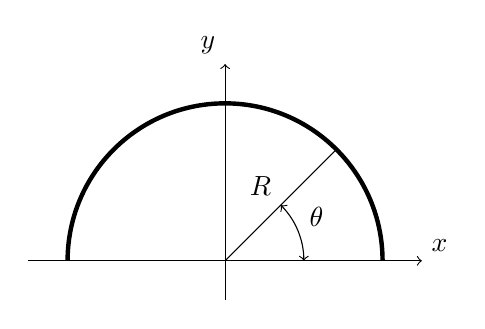
\begin{tikzpicture}[scale=0.5]
    \draw[black, ->] (-5,0) -- (5,0) node[black,anchor=south west] {$x$};
    \draw[black, ->] (0,-1) -- (0,5) node[black,anchor=south east] {$y$};
    \draw[black, ultra thick] (4,0) arc (0:180:4);
    \draw[black] (45:4) -- (0:0) node[black, pos=0.5, anchor=south east] {$R$};
    \draw[black, <->] (45:2) arc (45:0:2) node[black, pos=0.6, anchor=south west] {$\theta$};
\end{tikzpicture}
\end{figure}

Assuming the potential is zero at infinity, what is the total electric potential at the origin due to this charge distribution?

\end{frame}

\begin{frame}{Worked Example --- Potential of a Nonuniform Arc}

\textit{Solution.} The total electric potential at the origin can be found by integrating:
\begin{equation*}
    V = \int \frac{k\ dQ}{r}
\end{equation*}

We have a one-dimensional charge distribution, so
\begin{equation*}
    dQ = \lambda\ d\ell = \overbrace{\left( a \sin{\theta} \right)}^{\lambda} \overbrace{\left( R\ d\theta \right)}^{d\ell}
\end{equation*}

The magnitude of the $\vec{r}$-vector that appears in the integral above is simply $R$ (since that's the distance from the semicircle of charge to the origin).

\end{frame}

\begin{frame}{Worked Example --- Potential of a Nonuniform Arc}

Putting everything together gives us
\begin{align*}
    V = \int \frac{k\ dQ}{r} &= \int_{0}^{\pi} \frac{k\ \overbrace{\left( a\ \sin{\theta} \right)  \left( R\ d\theta \right)}^{dQ}}{R} \\[1em]
                             &= ka \int_{0}^{\pi} \sin{\theta}\ d\theta \\[1em]
                             &= \boxed{2ka} \blacktriangleleft
\end{align*}

\end{frame}

\begin{frame}{Relationship Between Voltage and Field}

Electric potential and electric field are related by a derivative:
\begin{equation*}
    E_x = -\frac{dV}{dx}
\end{equation*}

More generally,
\begin{equation*}
    \vec{E} = -\nabla V = -\frac{\partial V}{\partial x}\ihat - \frac{\partial V}{\partial y}\jhat - \frac{\partial V}{\partial z} \khat
\end{equation*}

For example, we know the potential of a point charge is $V = \frac{k q}{r}$. So the radial component of the electric field is
\begin{equation*}
    E_r = -\frac{\partial V}{\partial r} = - \left( - \frac{k\ q}{r^2} \right) = \frac{k\ q}{r^2}
\end{equation*}

\end{frame}

\begin{frame}{General Relationships Among Energy, Potential, Field, and Force}

\begin{figure}[H]
\centering
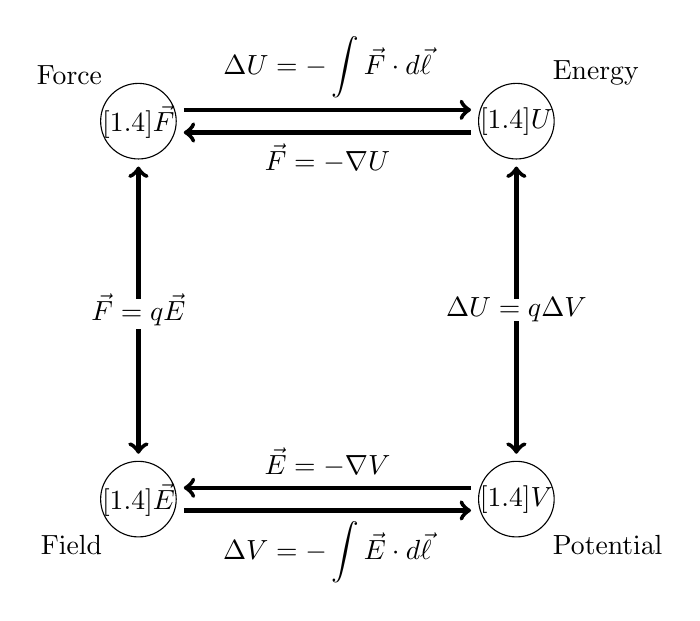
\begin{tikzpicture}[scale=0.48]
    % Nodes
    \draw[white] (5,5) -- (5.707,5.707) node[black, anchor=south west] {Energy};
    \draw[black] (5,5) circle (1);
    \node[black] at (5,5) {$\displaystyle \Scale[1.4]{U}$};
    \draw[white] (-5,5) -- (-5-0.707,5.707) node[black, anchor=south east] {Force};
    \draw[black] (-5,5) circle (1);
    \node[black] at (-5,5) {$\displaystyle \Scale[1.4]{\vec{F}}$};
    \draw[white] (-5,-5) -- (-5.707,-5.707) node[black, anchor=north east] {Field};
    \draw[black] (-5,-5) circle (1);
    \node[black] at (-5,-5) {$\displaystyle \Scale[1.4]{\vec{E}}$};
    \draw[white] (5,-5) -- (5.707,-5-0.707) node[black, anchor=north west] {Potential};
    \draw[black] (5,-5) circle (1);
    \node[black] at (5,-5) {$\displaystyle \Scale[1.4]{V}$};
    % Top Arrow
    \draw[black, ultra thick, ->] (-3.8,5.3) -- (3.8,5.3) node[black, midway, above] {$\displaystyle \Delta U = -\int \vec{F} \cdot d\vec{\ell}$};
    \draw[black, ultra thick, <-] (-3.8,4.7) -- (3.8,4.7) node[black, midway, below] {$\displaystyle \vec{F} = -\nabla U$};
    % Bottom arrow
    \draw[black, ultra thick, ->] (-3.8,-5.3) -- (3.8,-5.3) node[black, midway, below] {$\displaystyle \Delta V = -\int \vec{E} \cdot d\vec{\ell}$};
    \draw[black, ultra thick, <-] (-3.8,-4.7) -- (3.8,-4.7) node[black, midway, above] {$\displaystyle \vec{E} = -\nabla V$};
    % Right arrow
    \draw[black, ultra thick, <-] (5,3.8) -- (5,0.3);
    \node[black] at (5,0) {$\displaystyle \Delta U = q\Delta V$};
    \draw[black, ultra thick, ->] (5,-0.3) -- (5,-3.8);
    % Left arrow
    \draw[black, ultra thick, <-] (-5,3.8) -- (-5,0.3);
    \node[black] at (-5,0) {$\displaystyle \vec{F} = q \vec{E}$};
    \draw[black, ultra thick, ->] (-5,-0.5) -- (-5,-3.8);
\end{tikzpicture}
\end{figure}

\end{frame}

\begin{frame}{Worked Example --- Field From Potential}

$\blacktriangleright$ Suppose the electric potential in some region of space is given as $V(x, y, z) = 2.0 x^5 y^3 + 4.0 e^{5z}$. What is the $z$-component of the electric field?

\vfill

\textit{Solution.} Recall that 
\begin{equation*}
    \vec{E} = -\nabla V = -\frac{\partial V}{\partial x}\ihat - \frac{\partial V}{\partial y}\jhat - \frac{\partial V}{\partial z} \khat
\end{equation*}

So the $z$-component of the electric field is
\begin{equation*}
    E_z = - \frac{\partial V}{\partial z} = -20.0 e^{5z}
\end{equation*}

evaluated at the appropriate location. $\blacktriangleleft$

\end{frame}

\begin{frame}{Visualizing Electric Fields and Potentials}

Here's a term that's used all the time in electrostatics: \emph{equipotentials}. Recall that an equipotential line denotes a line where voltage is constant (much like contour lines on a topographical map).

\vfill

There's a phrase that helps me out a ton when thinking about potential and fields:

\begin{center}
    \emph{Electric field lines point downhill with respect to voltage.}
\end{center}

But that's a little too abstract. Let's see what that means in real life.

\end{frame}

\begin{frame}{Electric Field and Potential Visualized}

Suppose a have a \emph{dipole}. (This is nothing more than a positive and negative point charge separated some distance.)

\begin{figure}[H]
\centering
\includegraphics[height=0.5\textheight]{figures/dipole_field.png}
\end{figure}

This dipole system will make a field like that depicted above. But what about the potential? What does that look like?

\end{frame}

\begin{frame}{Electric Field and Potential Visualized}

The equipotential lines are \emph{normal} to the electric field lines.

\begin{figure}[H]
\centering
\includegraphics[height=0.5\textheight]{figures/dipole_potential.png}
\end{figure}

We can think of the positive charge kind of like a hill, and the negative charge kind of like a valley. Now observe how the electric field lines flow \emph{downhill} with respect to the equipotential lines. (This is the negative sign in the equation $\vec{E} = -\nabla V$.)

\end{frame}

\end{document}
